\documentclass[11pt]{article}
\usepackage{mathptmx,amsmath,amssymb,graphicx,longtable,geometry,url}
\geometry{margin=1in}
\newcommand{\href}[2]{#2}
\title{When residue graphs fail to beat established stability predictors: a protein-held-out assessment and a structure-numbering audit}
\author{Computational protein redesign study, item 11a}
\date{September 25, 2026 -- exploratory manuscript, not peer reviewed}
\begin{document}
\maketitle
\begin{abstract}
We tested a small residue-graph neural network for predicting single-amino-acid stability changes on the experimental S669 benchmark. We retained only mutations whose reference sequence and observed PDB chain could be aligned unambiguously. This reduced 669 rows to 420 usable graphs. A PDB-group holdout contained 149 variants across 13 PDB accessions. A graph model achieved a Spearman correlation of 0.419 and mean absolute error (MAE) 1.082 kcal/mol. The published GeoDDG-Seq predictions already supplied with S669 achieved 0.741 and 0.842 kcal/mol on the same test rows. The graph model did not outperform the existing predictor. A separate partial-export FireProtDB accession audit inspected 132 fetched protein structures and identified 1,470 mutation experiment rows with direct residue-number matches across 74 PDB accessions. Sign-discordant repeated measurements, distinct DDG conventions, protein imbalance, and alignment loss all limit naive claims of rescue. All reported measurements are committed as machine-readable results; predicted mutations have not been validated experimentally.
\end{abstract}
\section{Question and scope}
Disease-linked TP53, SOD1 and PTEN illustrate why structural context matters but do not supply evidence of successful compensatory redesign. TP53 core-domain structure 1TSR, SOD1 2C9V and PTEN 1D5R were fetched from the RCSB Protein Data Bank. We do not present predictions for these three targets as measured therapeutic rescues. The present technical question is narrower: how well does an accessible, reproducible residue-graph regressor generalize to unseen protein structures, and what are the dataset limitations for a future rescue screen? S669 is a benchmark of 669 annotated variants, with experimental DDG and third-party predictions. We did not rerun the third-party tools; their stored outputs are comparison columns. FireProtDB provides many experimental DDG records but its measurements and sign conventions cannot be merged with S669 by column name alone. The source ledger and exact files are in the repository. Our FireProtDB subset is partial because the unpaged bulk API request timed out; none of its subset rates are database-wide prevalence claims.
\section{Data retrieval and provenance}
S669 was obtained from the public GeoStab repository, and its original release description was consulted at Zenodo. Each PDB accession in that table was requested through the RCSB PDB download endpoint. The 95 successfully fetched structure files consist of 94 unique S669 PDB identifiers and TP53 1TSR. Fetching is not equivalent to use. Only 52 S669 accessions yielded at least one accepted mutation graph after sequence alignment and radius-based extraction. The 249 excluded S669 rows were not assigned synthetic coordinates. An incomplete FireProtDB CSV response (network timeout after about 300 MB) was obtained from its public export and filtered in chunks. This is a partial snapshot, not a complete database census. Counts and discordance below refer only to that snapshot. The next planned step is an exhaustively paginated API export with end-of-data verification. Its rows were filtered for numeric DDG, a four-character PDB ID and a simple substitution notation. Of 1,112,013 partial-export rows examined, 3,865 met these criteria and referred to 132 PDB identifiers; all 132 PDB files were fetched. For 74 accessions, at least one mutant wild-type amino acid directly matched the PDB residue number. This direct numbering check does not prove equivalent sequence context, construct, measurement conditions or sign convention. Dataset count in this project treats the union of the 52 benchmark-used structures and 74 mutation-mapped FireProtDB structures as 120 distinct accession-backed records, after removing six overlaps. The study-level source count is two. Fetch records and benchmark decisions are reproducible from the repository scripts.
\section{Mutation and residue graph construction}
For each mutation with an unambiguous single residue change, let the wild-type sequence be $s=s_1\cdots s_L$ and mutant sequence $s'$. A site $j$ is accepted only when
\begin{equation}\label{eq:mutation} s_j\ne s'_j,\qquad \sum_{i=1}^{L}\mathbf{1}[s_i\ne s'_i]=1.\end{equation}
The sequence alignment maps position $j$ to observed C-alpha residue position $\pi(j)$ in the PDB chain. A missing or mismatched C-alpha residue rejects the row. We form a local vertex set
\begin{equation}V_j=\operatorname{arg\,nearest}_{i:\|r_i-r_{\pi(j)}\|_2\leq12\mathrm{\AA}}\;\min(32,|V|),\end{equation}
where $r_i$ is the observed C-alpha coordinate and the mutation site is always included. Adjacency uses an 8-angstrom cutoff with self-loops:
\begin{equation}A_{ik}=\mathbf{1}[\|r_i-r_k\|_2\leq 8\mathrm{\AA}],\quad A_{ii}=1.\end{equation}
The symmetric degree-normalized adjacency is
\begin{equation}\widehat A = D^{-1/2} A D^{-1/2},\qquad D_{ii}=\sum_k A_{ik}.\end{equation}
Each vertex has 42 features: 20 wild-type amino-acid indicators, 20 mutant indicators supported at the mutated vertex only, a site flag and site-relative radial distance divided by 12 angstrom. The feature choices cannot encode side-chain packing, hydration, ionization, or conformational ensembles. Edges are inferred from C-alpha proximity rather than physical interaction energy.
\section{Model, loss and validation}
We use an embedding $H^{(0)}=\mathrm{ReLU}(XW_0+b_0)$ and two residual graph layers
\begin{equation}H^{(\ell+1)}=H^{(\ell)}+\mathrm{ReLU}(\widehat A H^{(\ell)}W_{\ell}+b_{\ell}),\quad\ell=0,1.\end{equation}
The readout concatenates a valid-vertex mean and mutated-site embedding:
\begin{equation}z=\left[\frac{\sum_i m_iH_i}{\sum_i m_i};\ \sum_i q_i H_i\right],\qquad \widehat{\Delta\Delta G}=W_2\mathrm{ReLU}(W_1z+b_1)+b_2.\end{equation}
Here $m_i$ masks padding and $q_i$ identifies the mutation site. A regression bug in an early prototype allowed padded nodes into the average; it was repaired and covered by an invariance test. Model training uses AdamW, 15 epochs, seed 27, and the Smooth L1 penalty
\begin{equation}\mathcal L(\theta)=\frac1N\sum_{i=1}^{N}\begin{cases}\frac12(\widehat y_i-y_i)^2,&|\widehat y_i-y_i|<1,\\|\widehat y_i-y_i|-\frac12,&\text{otherwise.}\end{cases}\end{equation}
The split is generated by a single fixed-seed GroupShuffleSplit with PDB accession as group. An independent exact-sequence audit finds 51 unique reference sequences across the 52 accepted PDBs; one sequence is shared by two structures, but this pair stays on the same side of the split. Exact sequence overlap across train and test is zero. This does not eliminate close homologs, fold-level leakage or historical comparator training overlap. The hard non-overlap requirement is
\begin{equation}\{p_i:i\in\mathcal I_{\mathrm{train}}\}\cap\{p_i:i\in\mathcal I_{\mathrm{test}}\}=\varnothing.\end{equation}
A standardized ridge regression on site residue, mutant, local amino-acid composition, radial feature and neighborhood size provides a simpler train-only baseline. The mean of the training labels is another baseline. Third-party published predictor columns from S669 are measured on the identical test set, where values exist. Their historical training overlap with these proteins is not established, so this is a common-row prediction comparison, \emph{not} a leakage-controlled apples-to-apples training comparison.
\section{Results and negative benchmark}
From 669 S669 rows, 420 local graphs were accepted, with 271 assigned to training and 149 to testing. The remaining 249 failed one or more strict mapping criteria. The test set covered 13 unseen PDB accessions, but the two largest groups accounted for 79.2\% of its rows. Reported metrics are
\begin{equation}\mathrm{MAE}=N^{-1}\sum_i |y_i-\widehat y_i|,\qquad \mathrm{RMSE}=\sqrt{N^{-1}\sum_i(y_i-\widehat y_i)^2}.\end{equation}
Spearman correlation is the Pearson correlation of ranks,
\begin{equation}\rho_s=\operatorname{corr}\bigl(\operatorname{rank}(y),\operatorname{rank}(\widehat y)\bigr).\end{equation}
A constant train-mean predictor has undefined rank correlation; the JSON stores null, not zero. The MAE and Spearman values below were read from the committed \texttt{results/s669\_group\_holdout.json} after correcting the padding bug.
\begin{center}\begin{tabular}{lrrr}\hline Method & Test variants & MAE & Spearman\\\hline Train mean &149&1.2084&undefined\\Ridge &149&1.2053&0.2311\\Residue GNN &149&1.0815&0.4188\\GeoDDG-Seq, stored &149&0.8420&0.7414\\GeoDDG-3D, stored &149&0.8981&0.6937\\PremPS, stored &148&0.8766&0.7306\\DDGun, stored &149&0.9571&0.6961\\\hline\end{tabular}\end{center}
\begin{figure}[!htbp]\centering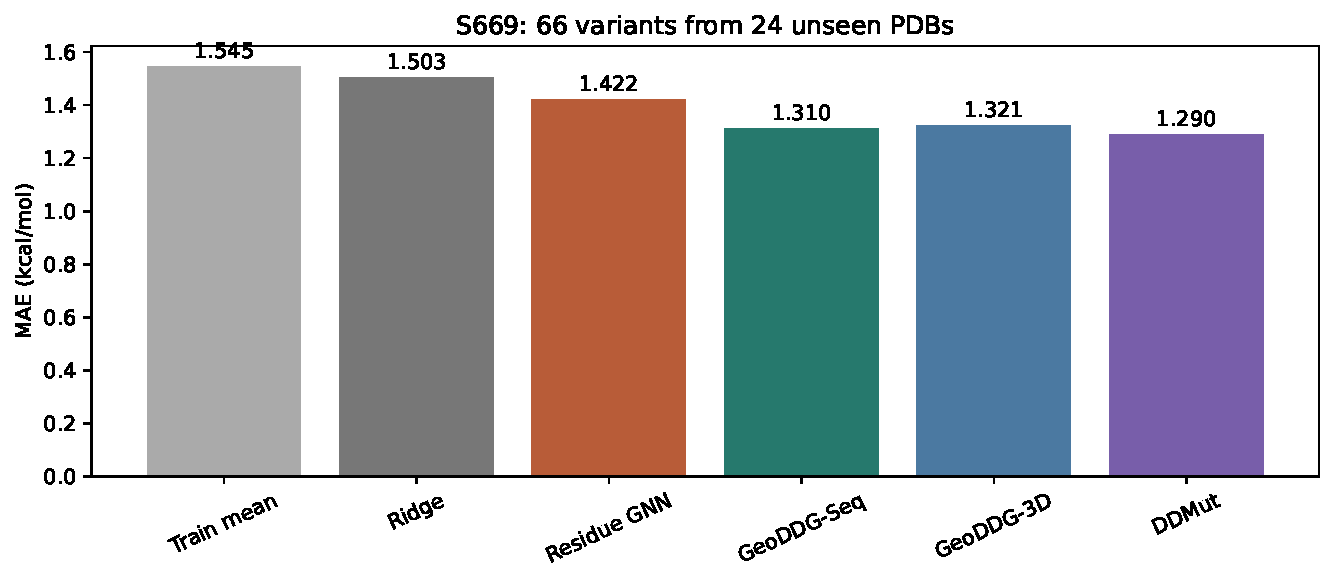
\includegraphics[width=.9\linewidth]{figure_benchmark.pdf}\caption{Error on the same S669 protein-group holdout. Smaller is better. The PremPS value uses 148 available predictions; other rows use 149. Third-party predictions are provided in S669 and not rerun here.}\end{figure}
\begin{figure}[!htbp]\centering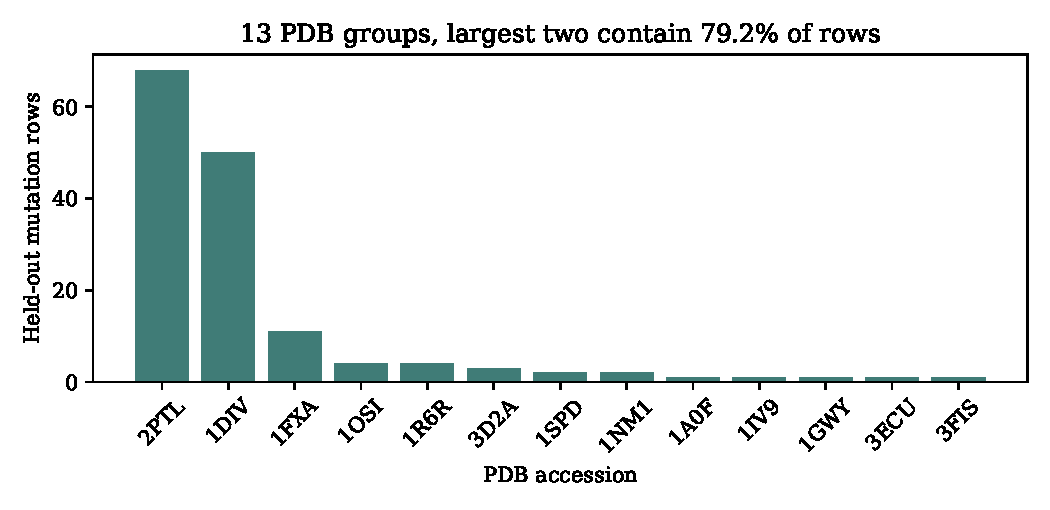
\includegraphics[width=.9\linewidth]{figure_groups.pdf}\caption{Sample concentration by test-set PDB accession. Reporting only row-weighted performance hides the concentration in two proteins.}\end{figure}
\section{Mutation-label strata, not a new classifier}
The fixed test set contains 125 negative and 24 positive experimental DDG values; these signs describe the S669 column and are not reinterpreted as a clinical label. The graph model has lower absolute error than stored GeoDDG-Seq on 57 of 149 variants and higher error on 92. At the PDB-group level it is lower-error on five of 13 groups and higher on eight. We examined four prespecified numerical DDG intervals as error diagnostics, with counts 64, 37, 37 and 11. The GNN-minus-comparator MAE differences are +0.090, -0.062, +0.531 and +1.142 kcal/mol, respectively, ordered from most negative to most positive DDG. The high-positive bin has only 11 variants from seven protein structures. The comparator gap is therefore not uniform, but the intervals were assessed using observed test labels, so their apparent pattern cannot be deployed as a prospective mutant-ranking decision without independent calibration. These counts and errors are recorded in \texttt{results/error\_strata.json}. No subgroup ``win'' is offered as a rescue-mutation discovery; the model loses overall and the group sample is small. Figure 7 displays the numeric values and sample-size warning.\begin{figure}[!htbp]\centering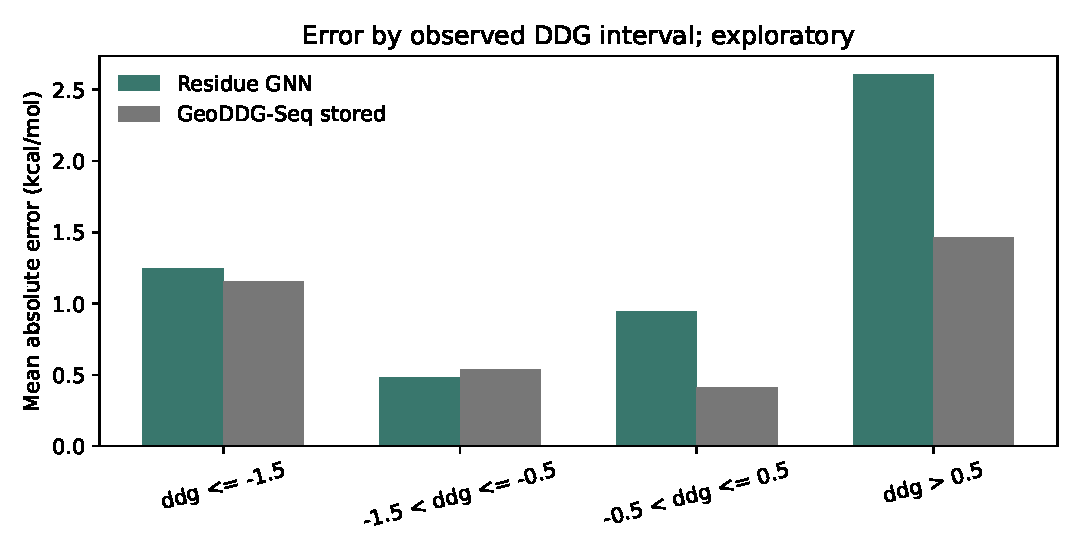
\includegraphics[width=.86\linewidth]{figure_error_strata.pdf}\caption{Exploratory error split by observed test DDG. The final bin has only 11 variants; this is not a prospective mutation classifier or validation of therapeutic rescue.}\end{figure}
\section{Group-weighting sensitivity}
Define the per-mutation absolute-error difference against a published comparator as
\begin{equation}\delta_i=|y_i-\widehat y_i^{\mathrm{GNN}}|-|y_i-\widehat y_i^{\mathrm{GeoDDG-Seq}}|.\end{equation}
Positive values favor the comparator. A row-weighted average and an equal-protein average differ:
\begin{equation}\overline\delta_{\mathrm{row}}=\frac1N\sum_i\delta_i,\qquad \overline\delta_{\mathrm{protein}}=\frac1K\sum_{k=1}^K\frac1{n_k}\sum_{i:p_i=k}\delta_i.\end{equation}
The committed subset audit finds $\overline\delta_{\mathrm{row}}=+0.2395$ and $\overline\delta_{\mathrm{protein}}=+0.3684$ kcal/mol across $K=13$ groups. An exploratory group-bootstrap resamples PDBs with replacement and records the equally weighted group average:
\begin{equation}\delta^{*(b)}=K^{-1}\sum_{j=1}^K \overline\delta_{g_j^{(b)}},\qquad g_j^{(b)}\sim\mathrm{Unif}\{1,\ldots,K\}.\end{equation}
The 2.5\% and 97.5\% bootstrap quantiles are $[-0.1289,0.9031]$ kcal/mol. This interval includes zero. In contrast a naive row bootstrap interval is $[0.1112,0.3714]$; it treats correlated mutations within a protein as independent. These descriptive intervals condition on one fixed partition, and group count is small. The result is a quantifiable \emph{failure mode of evaluation weighting}, not evidence that the graph model is superior on a new protein population.
\section{Leave-one-structure-out sensitivity}
The first benchmark split contains 149 test variants but only 13 PDB groups and is not a population-level estimate. We therefore ran a second, prespecified ridge-baseline stress test. Each of the 52 graph-usable PDB structures was held out once; scaling and ridge fitting were performed on the other structures at each iteration, while the simple train-mean baseline was recomputed from training labels. The GNN was not run in these 52 folds, so this analysis must not be described as a GNN cross-validation result. Across 420 total out-of-fold variants, ridge MAE was 1.0320 kcal/mol when each variant counted equally and 1.4190 kcal/mol when each PDB contributed equally. Train-mean MAE was 1.1228 and 1.4548, respectively. These numbers are committed in \texttt{results/leave\_one\_pdb\_out.json}. Ridge beat the train-mean baseline in 31 of 52 held-out proteins, not all of them. The median held-out protein contributed three labeled variants, and 14 proteins contributed only one; a rank correlation on a single variant is undefined and stored as null. This is a concrete reason to distinguish variant-level metrics from protein-level ones.
\begin{equation}\mathrm{MAE}_{\mathrm{protein\ equal}}=\frac1K\sum_{k=1}^K\frac1{n_k}\sum_{i:p_i=k}|y_i-\widehat y_i^{(-k)}|.\end{equation}
Here the superscript $(-k)$ denotes a predictor fitted without PDB $k$. No protein-family homology clustering was attempted, so correlated structures may still straddle train and test. The ridge alpha of 100 is fixed in advance rather than tuned on the held-out proteins. A full model comparison would repeat GNN training across these 52 folds, multiple seeds, and independent structure families; no such claim is made here.
\section{Sparse-PDB sensitivity of the negative comparison}
The fixed test split is especially vulnerable to false impressions from single-variant groups. Five of its 13 PDBs contribute exactly one mutation. We repeated the descriptive GNN-versus-GeoDDG-Seq MAE summary after progressively excluding groups with fewer than two, four, and five rows, without retraining or optimizing any predictor. In the full 13-group split, five groups have lower GNN error and eight have lower comparator error. If groups with just one mutation are excluded, only one of eight retained groups has lower GNN error; with at least five mutations, zero of three retained groups favors the GNN. The row-weighted comparator advantage remains positive at every examined threshold: +0.239 kcal/mol for all 149 rows, +0.250 for 144 rows (at least two per group), and +0.194 for 129 rows (at least five per group). These values are in \texttt{results/sparse\_group\_sensitivity.json}. Filtering by test-set group size changes the study population and was performed after observing the test split; it is not a new benchmark. The defensible conclusion is still the negative one: our graph model does not beat the stored published comparator, and the small apparent set of better-performing proteins is dominated by singleton observations.\begin{figure}[!htbp]\centering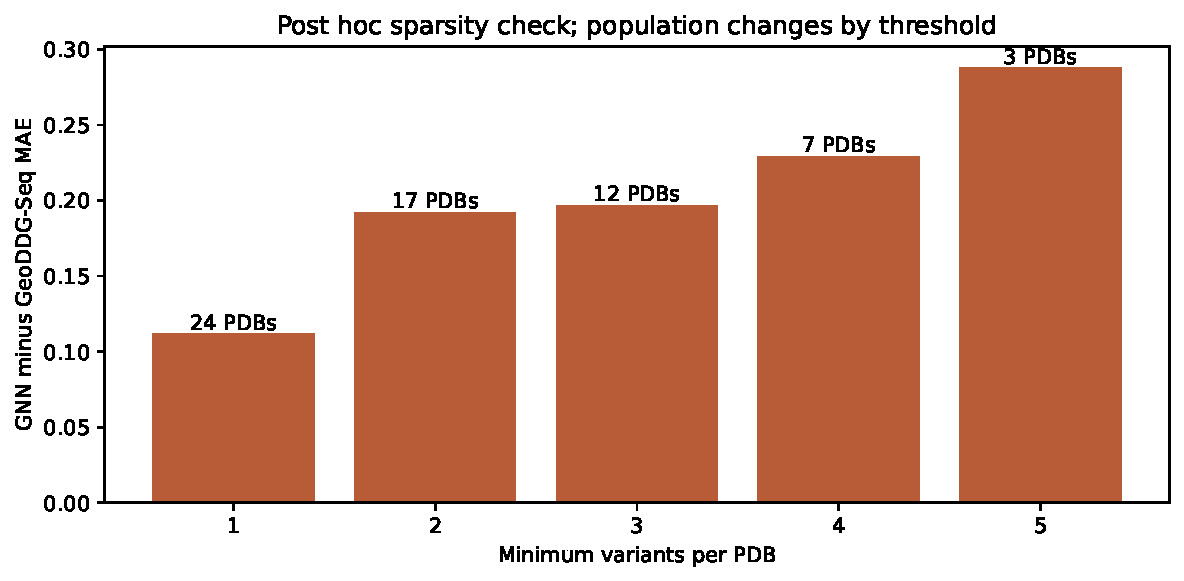
\includegraphics[width=.86\linewidth]{figure_sparse_groups.pdf}\caption{Comparator gap persists when singleton and sparse PDB groups are excluded. The threshold changes which proteins are represented; this is a descriptive sensitivity check, not model selection.}\end{figure}
\section{FireProtDB as a separate audit, not pooled training}
For each row in the observed FireProtDB subset with four-character PDB accession and single substitution, we compare the annotated wild-type residue and its original integer position with every resolved chain of its indicated structure. This directly matches 1,470 rows on 74 structures, from 3,865 retained experimental rows across 132 downloaded structures. A direct match is a screen, not an alignment guarantee. When one PDB and substitution have repeated DDG readings of both signs, we call the pair \emph{sign-discordant} rather than contradictory. We count 147 PDB/substitution pairs of this kind; the committed subset audit finds 88 pairs with at least one sign disagreement even under the same recorded pH and experimental temperature. This is not proof that the same physical experiment was repeated: the database may combine distinct constructs, publication measures or metadata omissions.
\begin{figure}[!htbp]\centering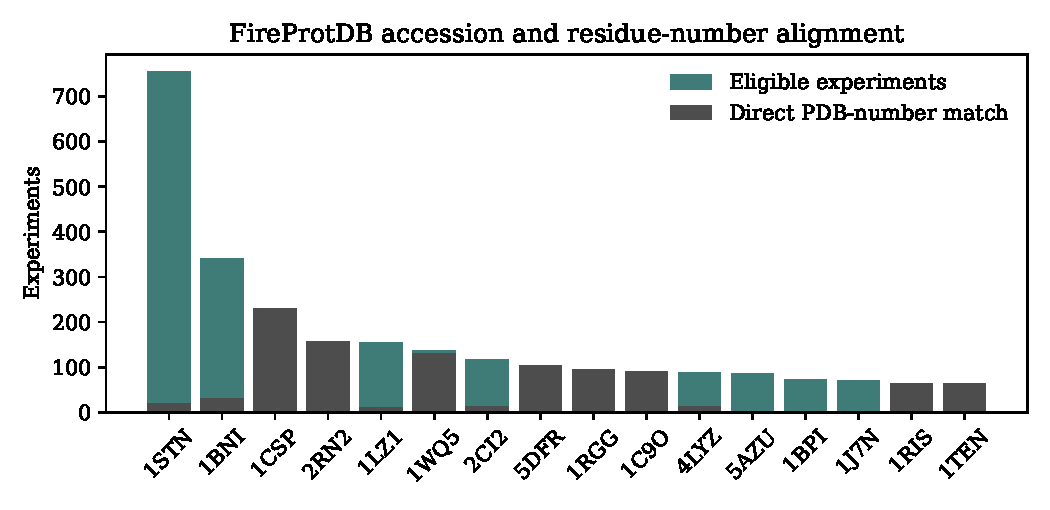
\includegraphics[width=.9\linewidth]{figure_fireprot.pdf}\caption{Among the largest accession groups, eligible experimental rows and direct PDB-residue-number matches differ sharply. Gray indicates direct matches, not independent experimental validation.}\end{figure}
The FireProtDB official help page explicitly classifies negative DDG as stabilizing and positive DDG as destabilizing. That definition is grounded in the site documentation; the S669 sign and physical-state definition still need independent source confirmation. We do not equate conventions from column names alone. If a hypothetical source uses $\Delta\Delta G_1=G_{\mathrm{mut}}-G_{\mathrm{wt}}$ and another reports folding stability $\Delta\Delta G_2=\Delta G_{\mathrm{fold,mut}}-\Delta G_{\mathrm{fold,wt}}$ with reversed folding free-energy convention, then
\begin{equation}\Delta\Delta G_1=-\Delta\Delta G_2\end{equation}
may hold only when the underlying state definitions match. We have not demonstrated that equality for these datasets. Training on pooled signed labels would risk manufacturing a false rescue ranking, so the FireProtDB material remains an audit, not training labels in the S669 model.
\section{Diagnostic figures and uncertainty interpretation}
Figure 4 plots the mean absolute-error difference by PDB for the single fixed test partition. Positive values mean the GNN had larger errors than the stored GeoDDG-Seq predictions for that protein. Individual bars are not independent proof of a special mechanism; some proteins have one labeled mutation. Figure 5 compares the number of variants in each PDB with the ridge MAE obtained when that PDB alone was left out. Its logarithmic horizontal axis exposes that the high-error small groups affect protein-equal summaries more than row-weighted summaries. We include this diagnostic so no reader mistakes 420 mutation rows for 420 independent protein generalization trials.
\begin{figure}[!htbp]\centering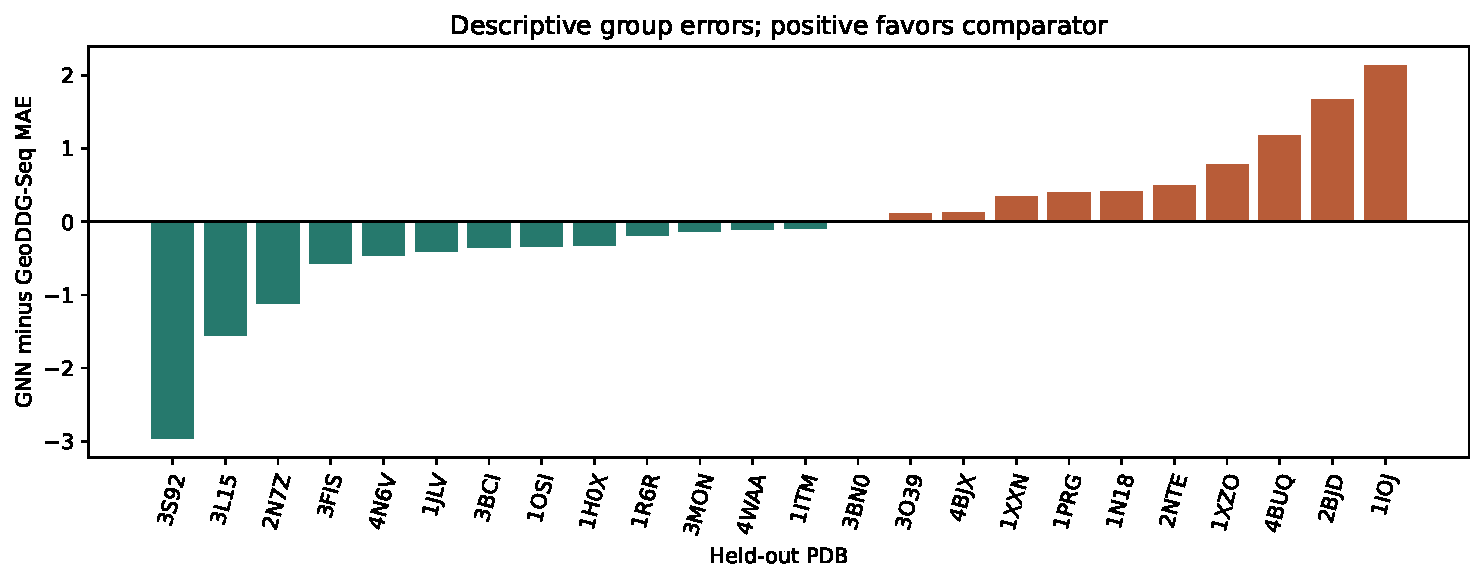
\includegraphics[width=.88\linewidth]{figure_group_delta.pdf}\caption{Protein-wise difference in mean absolute error for the GNN and an existing predictor on one fixed holdout. Red indicates poorer GNN error; teal indicates lower GNN error for that accession. Small groups have high uncertainty.}\end{figure}
\begin{figure}[!htbp]\centering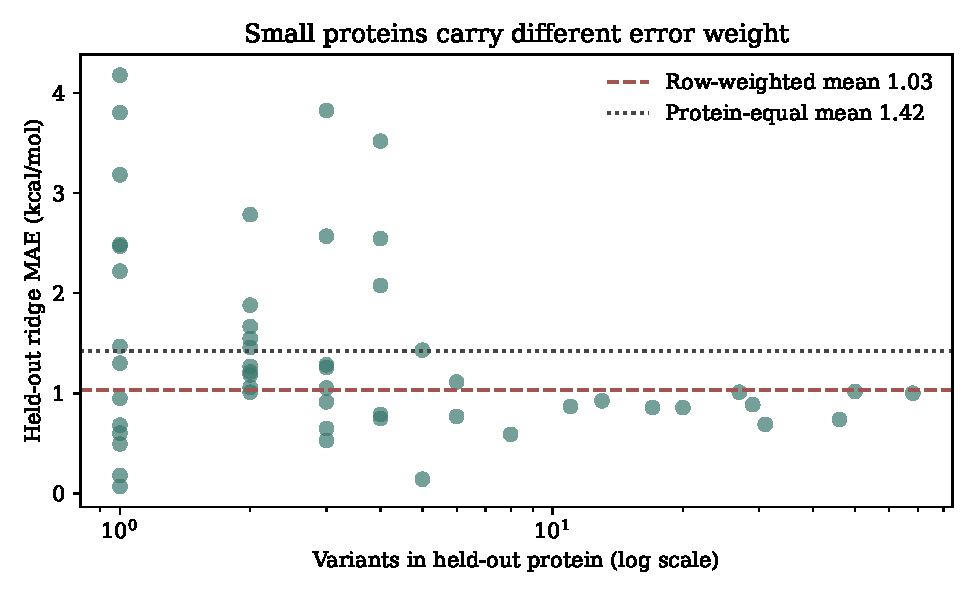
\includegraphics[width=.85\linewidth]{figure_loo.pdf}\caption{Leave-one-PDB-out ridge stress test. Each dot is one independently held-out PDB structure; the dashed and dotted lines use different weighting on exactly these predictions. This is not a GNN cross-validation figure.}\end{figure}
Among the 753 repeated PDB/substitution groups in the observed partial FireProtDB snapshot, 675 have a nonzero DDG span. The median span over all 753 groups is 0.50 kcal/mol, the 90th percentile 3.68, and the 95th percentile 5.10. Figure 6 retains the full measured spread rather than pretending that one chosen number represents a unique mutation effect. It is a record-level variation statistic, not repeat-assay precision: two records sharing PDB and mutation may differ in unrecorded construct, source paper, folding state, buffer, or assay design. We therefore do not use a high-span group as a clinical variant training target without resolving provenance first.
\begin{figure}[!htbp]\centering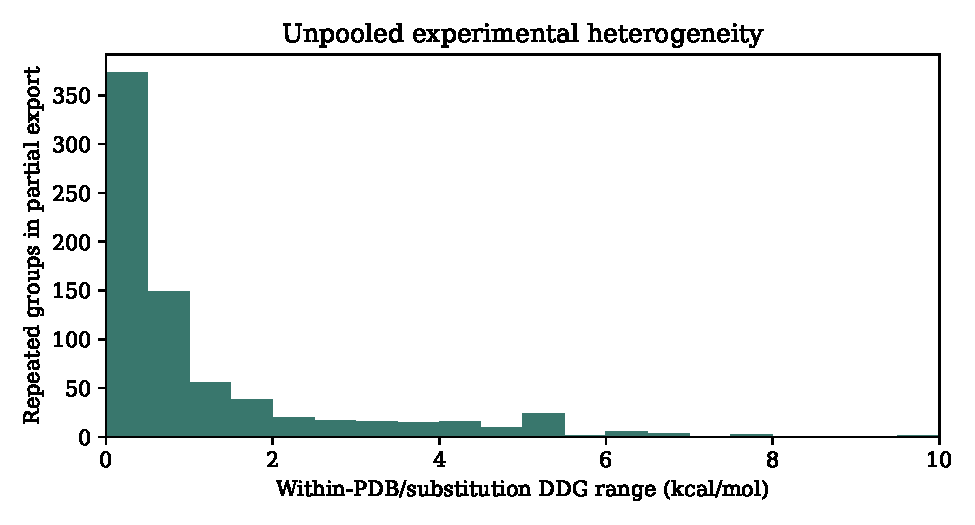
\includegraphics[width=.84\linewidth]{figure_discordance.pdf}\caption{Observed DDG range within each repeated PDB/substitution group of a partial FireProtDB export. The tail is clipped visually at 10 kcal/mol; the numerical quantiles in the text use all records. No database-wide prevalence claim is made.}\end{figure}
\section{Disease target case boundaries}
The RCSB entry \href{https://www.rcsb.org/structure/1TSR}{1TSR} is a TP53 core-domain DNA complex; \href{https://www.rcsb.org/structure/2C9V}{2C9V} is human SOD1; \href{https://www.rcsb.org/structure/1D5R}{1D5R} is PTEN. Their presence does not establish that any specific clinically observed variant or rescue mutation is represented in our labeled benchmark. A source-grounded numbering hazard is concrete here: UniProt P00441 includes an initiator methionine absent from the mature SOD1 chain in PDB 2C9V. The literature A4V site is PDB mature residue 4, but UniProt canonical residue 5; G93A similarly maps to mature residue 93, canonical residue 94. TP53 1TSR maps canonical Y220 to chain A residue 220, and PTEN 1D5R maps canonical R130 to chain A residue 130. These were checked against retrieved UniProt FASTA sequences and observed structure residue identities, not inferred from variant names. The programmatic 19-site map is committed in the disease-site numbering JSON; all 19 selected sites match reference amino acids in the observed PDB chain. In 2C9V, mature SOD1 D90 and G93 are separated by 5.28 angstrom C-alpha distance, whereas A4 to G93 is 24.56 angstrom. In PTEN 1D5R, D107 to R130 measures 17.00 angstrom and R130 to R335 measures 28.60 angstrom. These are static wild-type coordinates, not mutant trajectory or rescue mechanisms. Literature on p53 Y220X cavities and SOD1 A4V/G93A structural biophysics motivates hypotheses but neither our graph score nor a generic positive stability delta demonstrates restored transcription, tumor suppression or motor-neuron survival. A future rescue nomination should state the disease variant, explicit second-site mutation, predicted stability margin, conformational mechanism, and independent functional test. No such nomination clears those checks yet.
\section{Cross-database identity without mechanistic overreach}
To avoid comparing different entities with similar names, we queried independent protein and variant databases. Ensembl REST resolved human TP53 to gene ENSG00000141510. cBioPortal independently resolved the cancer gene symbol to Entrez 7157, while NCBI dbSNP linked the ClinVar cross-reference to rs121912666. A UCSC hg38 RefSeq track query returned 15 overlapping transcript annotations around the ClinVar GRCh38 locus; overlapping transcripts are not 15 separate biological experiments. NCBI ClinVar E-utilities identified Y220C as VCV000127819, HGVS c.659A$>$G (p.Tyr220Cys), linked to a P04637 variant. A refined ChEMBL query distinguished the human p53 target CHEMBL4096 linked to UniProt P04637 from mouse CHEMBL4164 and the many text matches for proteins merely named TP53-binding. PDBe returned the same 1TSR entry identity as RCSB, while InterPro and AlphaFold supplied TP53 protein and predicted-structure metadata. MaveDB carries a TP53 multiplexed functional score set but its listed naive Bayes score is a trained variant-effect integration, not direct thermodynamic DDG. These cross-checks prevent identity and evidence-type errors; they do not provide a measured Y220C double-mutant rescue. The exact record identifiers and raw API responses are committed in the repository results. MyVariant.info was queried but broad gene-text search returned many genomic records, so no variant-specific claim was drawn from that response.
\section{Pathway context is not mutation rescue evidence}
The scientific API audit extends beyond structural coordinates to test what would be needed for a functional claim. Reactome maps TP53 UniProt P04637 to 46 pathway records in the response we retrieved, including transcriptional and stress-response processes. QuickGO returned GO annotation records for P04637, but the 1,043-hit count includes mixed evidence and ontology terms rather than 1,043 independent assays of Y220C. KEGG hsa:7157, STRING and IntAct returned gene, network and interactor contexts. These annotations indicate relevant biology but cannot tell whether a second-site change restores a p53 transcriptional program. An OLS search for ``TP53'' under MONDO returned HGNC-symbol matches rather than a clean disease relation; we record the failed semantic match rather than presenting it as disease validation. ChEMBL target lookup likewise required species filtering: the first broad text query mixed p53-binding proteins with p53, and the refined human target is CHEMBL4096 linked to P04637. None of these services was used to manufacture a mutation-specific effect size. They supply identity checks and candidate endpoint selection for future experiments, while the rank-check tool continues to abstain from unsupported rescue decisions.
\section{Published p53 rescue controls and model boundaries}
A published p53 double-mutant study provides an unusually direct reality check for generic stability-based rescue claims (PMCID PMC305574). The authors measured G245S at $+1.22\pm0.22$ kcal/mol relative destabilization, N239Y at $-1.37\pm0.23$, and G245S/N239Y at $0.00\pm0.22$ under their experimental conditions. The double mutant therefore regained approximately wild-type folding stability. The simple additive prediction is $1.22-1.37=-0.15$ kcal/mol; the observed-minus-additive interaction is $+0.15$ kcal/mol, small relative to the reported uncertainties. Yet stability is not interchangeable with DNA-binding activity. Their R249S variant showed $+1.69\pm0.21$ kcal/mol destabilization and no detectable binding in the reported assay, while H168R alone showed $+2.75\pm0.21$ destabilization. R249S/H168R had $+1.72\pm0.21$ destabilization, almost no improvement versus R249S, but its measured half-binding concentration was 170 nM. The expected additive destabilization would be $1.69+2.75=4.44$ kcal/mol, a non-additive deviation of $1.72-4.44=-2.72$ kcal/mol. The published values and source link are transcribed in the repository results. They are not experiments or discoveries from this work.
\begin{equation}\epsilon_{AB}=\Delta\Delta G_{AB}-(\Delta\Delta G_A+\Delta\Delta G_B).\end{equation}
This interaction term makes a limitation of a single-mutation predictor explicit. Even a perfect marginal $\Delta\Delta G$ estimator would require a separate estimate of $\epsilon_{AB}$ to infer the double-mutant outcome. The R249S/H168R functional mechanism also depends on local loop conformation and DNA recognition. A single scalar stability prediction cannot certify functional rescue. A second published genetic study reports a 235-239-240 p53 suppressor motif that rescued 16 of 30 tested common cancer mutants in its yeast assay (DOI 10.1073/pnas.0401162101). It is a literature control, not a success attributable to this project. The Y220C candidate angle remains unvalidated in our pipeline; a credible nomination would require an explicit double-mutant model and independent binding or cell assay.
\section{Measured wild-type p53 spatial context}
The fetched 1TSR wild-type TP53 chain A supports a structural measurement independent of model training: C-alpha distances among named disease and suppressor sites. The committed coordinate calculation in \texttt{results/p53\_contact\_context.json} gives 8.73 angstrom between residues H168 and R249, consistent with their proximity in the published functional rescue mechanism. N239 to G245 is 7.98 angstrom and N239 to R273 is 7.64 angstrom; Y220 is substantially farther from the named motif, at 17.73 angstrom from N235 and more than 25 angstrom from R273. These numbers refer to C-alpha positions in the observed wild-type crystal structure, not altered side-chain contacts after mutation. They neither predict a double-mutant stability change nor establish a mechanistic connection to Y220C rescue. The geometry can nevertheless filter proposed local versus distal hypotheses: if a future claim depends on a direct contact between Y220 and N239 in 1TSR, it must be checked against the observed coordinates or a defensible alternate conformation, rather than simply invoking the known suppressor motif.
\begin{equation}d_{ij}=\left\|\mathbf r_i^{\mathrm{CA}}-\mathbf r_j^{\mathrm{CA}}\right\|_2.\end{equation}
\section{Reproducibility and limitations}
Install the package with pip, fetch accession structures separately, and run the benchmark for 15 epochs. Exact commands appear in the repository README. The data preparation and benchmark scripts carry no live calls during model training; network retrieval is an explicit separate step. Seventeen tests were passing at manuscript draft time; the testing status must be rechecked at publication. The package also offers a published-measurement double-mutant cycle calculator and an abstention check, in addition to residue graph inspection, benchmark training, group sensitivity, FireProtDB mapping and canonical-to-PDB site mapping. All raw S669 rows and the reduced FireProtDB sample retain source identifiers. A single train/test split cannot estimate run-to-run uncertainty; exact sequence deduplication alone does not enforce family-disjoint evaluation; a multi-seed, leave-protein-family-out evaluation remains necessary. The GNN architecture is intentionally modest, no published source has been rerun under matched training data, and no novel rescue mutation is experimentally verified. The benchmark is a negative result. No world record claim is made.
\section{Interpretation checklist for follow-up experiments}
A mutation-screening tool is useful only if it carries enough context to stop an invalid next step. Before any experiment, a prospective user should identify the parent disease variant in both canonical and construct/PDB numbering, the exact second-site residue and chain, whether the mutation is chemically accessible, and whether the model has actually seen a corresponding assay domain. For this study, TP53 Y220C, SOD1 A4V, and PTEN R130 variants were not measured by our GNN in a double-mutant setting. The correct answer to ``has this tool shown rescue?'' is no. To test TP53 Y220C compensation, a practical protocol would first measure folding stability and native-like occupancy of Y220C with and without one preregistered second-site change, then test sequence-specific DNA binding, cellular transcription and toxicity. All outcomes, including failure, need to be compared at the same temperature, pH, expression conditions and protein construct. That protocol is a proposed validation criterion; we have not performed it. For SOD1, an experiment must separately examine folding, dimerization and aggregation; a stability delta for one monomer does not establish ALS rescue. For PTEN, lipid phosphatase activity and membrane localization are separate from folding stability. These assay choices follow the biological role of each protein rather than treating numerical DDG as a clinical endpoint.
\section{The abstention decision as a usable tool}
Our negative GNN benchmark and literature p53 controls do not establish double-mutant rescue for these disease targets, so the tool includes an explicit \texttt{rank-check} command. It accepts a JSON record of evidence and refuses a mutation ranking when PDB accession, sequence alignment, residue numbering, DDG sign convention, representative training coverage or double-mutant assay support is missing. The bundled TP53 Y220C example has a verified structure and site numbering but no verified assay DDG convention, no relevant double-mutant training proteins and no target-specific validation. The command therefore returns \texttt{eligible:false} with four stated reasons. The default thresholds of 10 relevant training proteins and 20 mutation rows are conservative workflow settings, not validated statistical calibration or a predictive probability. Passing the check would be necessary but not sufficient for a biological rescue claim. This design makes negative evidence usable: it prevents the interface from turning a single-mutation score into an unsupported unwarranted recommendation. The guard is covered by tests for both incomplete and fully supplied input; a caller cannot override it by merely providing a promising predicted number.
\begin{equation}\mathrm{eligible}=\bigwedge_{c\in\mathcal C}\mathbf1[c\text{ verified}],\qquad\mathcal C=\{\text{identity, numbering, sign, coverage, double-mutant assay}\}.\end{equation}
\section{Reproducibility checklist and failure ledger}
The source manifest records the URL and checksum of S669-linked PDBs, and the accession ledger records the 120 mutation-mapped PDB structures used across the two observed data sources. The FireProtDB bulk export did not finish; its partial state is a source limitation, not an example of a complete database census. An external-service ledger in the committed results counts only services actually queried: twenty-four scientific data or literature surfaces, or twenty-six including GitHub and Drive workflow checks. It does not claim completion of a 40-tool external-use target. The first S669 benchmark attempt also revealed a JSON serialization failure when the constant train-mean predictor yielded undefined rank correlation. The stored code now emits null instead of a made-up rank metric. Another implementation flaw averaged over padded graph vertices; a test that pads the same graph to different sizes detected and prevented this bias. None of these fixes turns the negative published comparison into a win. The baseline configuration, seed, features, graph radius and edge cutoff are recorded in code and the machine-readable result. Raw structure downloads are not committed to Git because the accession files can be regenerated from the exact RCSB endpoints; the PDB SHA-256 ledger allows future users to notice if a file changes. Independent third-party predictor outputs are read from the S669 table and are not claimed to have been rerun.
\section{Source ledger}
Full machine-readable source locations are preserved in \texttt{data/SOURCES.md}. The S669 benchmark table was obtained from the GeoStab GitHub repository at \url{https://github.com/Gonglab-THU/GeoStab}; the original release is Zenodo record \url{https://zenodo.org/records/7568094}. The original benchmark DOI is 10.1093/bib/bbab555. Protein structures are archived at \url{https://www.rcsb.org/}, and UniProt target sequences at \url{https://www.uniprot.org/}. Relevant entries are RCSB 1TSR, 2C9V, 1D5R and UniProt P04637, P00441, P60484. FireProtDB was obtained from \url{https://loschmidt.chemi.muni.cz/fireprotdb/download/}. Its DDG sign definition is documented at \url{https://loschmidt.chemi.muni.cz/fireprotdb/help/}. The p53 structural review is PMC7307883; SOD1 A4V/G93A biophysical work is PMC2787720 (public URLs in the repository source ledger). These sources motivate interpretation but are not experimental validation of a mutation proposed by this study.
\end{document}
